\hypertarget{mtk__matrix_8cc}{\section{src/mtk\+\_\+matrix.cc File Reference}
\label{mtk__matrix_8cc}\index{src/mtk\+\_\+matrix.\+cc@{src/mtk\+\_\+matrix.\+cc}}
}


Implementing the representation of a matrix in the M\+T\+K.  


{\ttfamily \#include $<$cstdlib$>$}\\*
{\ttfamily \#include $<$cstdio$>$}\\*
{\ttfamily \#include $<$cstring$>$}\\*
{\ttfamily \#include $<$cmath$>$}\\*
{\ttfamily \#include $<$iomanip$>$}\\*
{\ttfamily \#include $<$iostream$>$}\\*
{\ttfamily \#include \char`\"{}mtk\+\_\+tools.\+h\char`\"{}}\\*
{\ttfamily \#include \char`\"{}mtk\+\_\+matrix.\+h\char`\"{}}\\*
Include dependency graph for mtk\+\_\+matrix.\+cc\+:\nopagebreak
\begin{figure}[H]
\begin{center}
\leavevmode
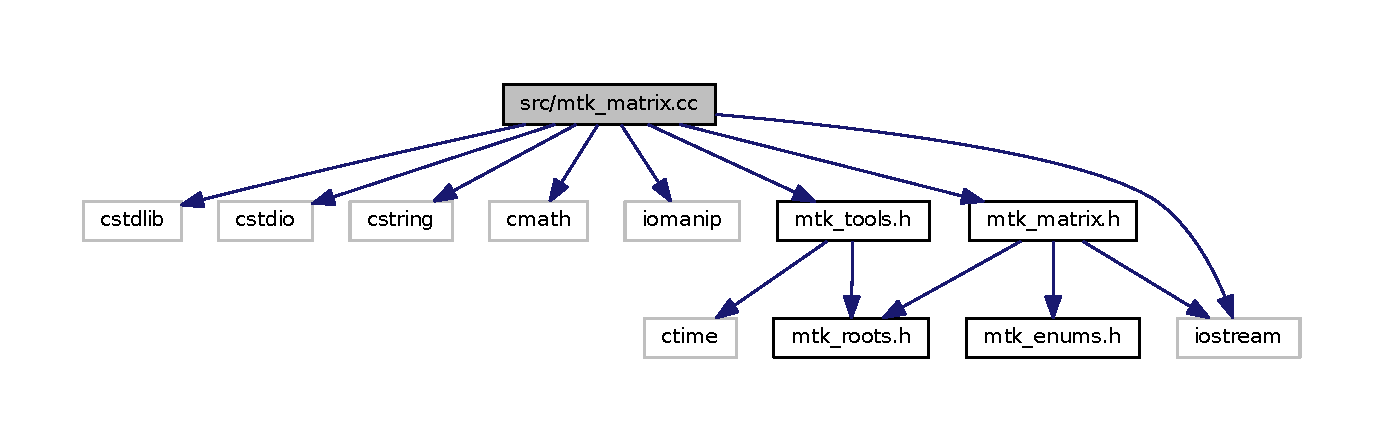
\includegraphics[width=350pt]{mtk__matrix_8cc__incl}
\end{center}
\end{figure}


\subsection{Detailed Description}
Implementation of the representation for the matrices implemented in the M\+T\+K.

\begin{DoxyAuthor}{Author}
\+: Eduardo J. Sanchez (ejspeiro) -\/ esanchez at mail dot sdsu dot edu 
\end{DoxyAuthor}


Definition in file \hyperlink{mtk__matrix_8cc_source}{mtk\+\_\+matrix.\+cc}.

